\documentclass[10pt]{article}
\usepackage[margin=0.45in]{geometry}
\usepackage{tikz}
\usepackage{amsmath}
\usepackage{booktabs}
\usepackage{array}
\usepackage{xcolor}
\usepackage{graphicx}
\usepackage{caption}
\usetikzlibrary{arrows.meta, positioning, fit, backgrounds, calc}
\pagestyle{empty}

\definecolor{inputblue}{RGB}{221,235,247}
\definecolor{histgreen}{RGB}{226,240,217}
\definecolor{latentorange}{RGB}{252,228,214}
\definecolor{odepurple}{RGB}{232,222,248}
\definecolor{decodeyellow}{RGB}{255,242,204}
\definecolor{graybox}{RGB}{242,242,242}
\definecolor{linegray}{RGB}{70,70,70}

\tikzset{
  block/.style={
    draw=linegray,
    rounded corners=2pt,
    align=center,
    minimum height=8mm,
    inner sep=4pt,
    font=\scriptsize
  },
  input/.style={block, fill=inputblue, minimum width=28mm},
  hist/.style={block, fill=histgreen, minimum width=33mm},
  latent/.style={block, fill=latentorange, minimum width=31mm},
  ode/.style={block, fill=odepurple, minimum width=35mm},
  decode/.style={block, fill=decodeyellow, minimum width=32mm},
  small/.style={block, fill=graybox, minimum width=25mm},
  group/.style={draw=linegray, rounded corners=3pt, dashed, inner sep=6pt},
  arrow/.style={-{Latex[length=2.2mm]}, line width=0.45pt, draw=linegray},
  label/.style={font=\tiny, align=center, fill=white, inner sep=1pt}
}

\begin{document}

\begin{center}
{\Large NODE2 Full-Upgrade Network Architecture}\\[2mm]
{\small ANUGA h3 run: $H=3$, $F=64$, $D_s=4$, $D_u=1$, $D_y=3$, $D_e=D_h=D_z=96$}
\end{center}

\begin{figure}[h!]
\centering
\resizebox{\textwidth}{!}{%
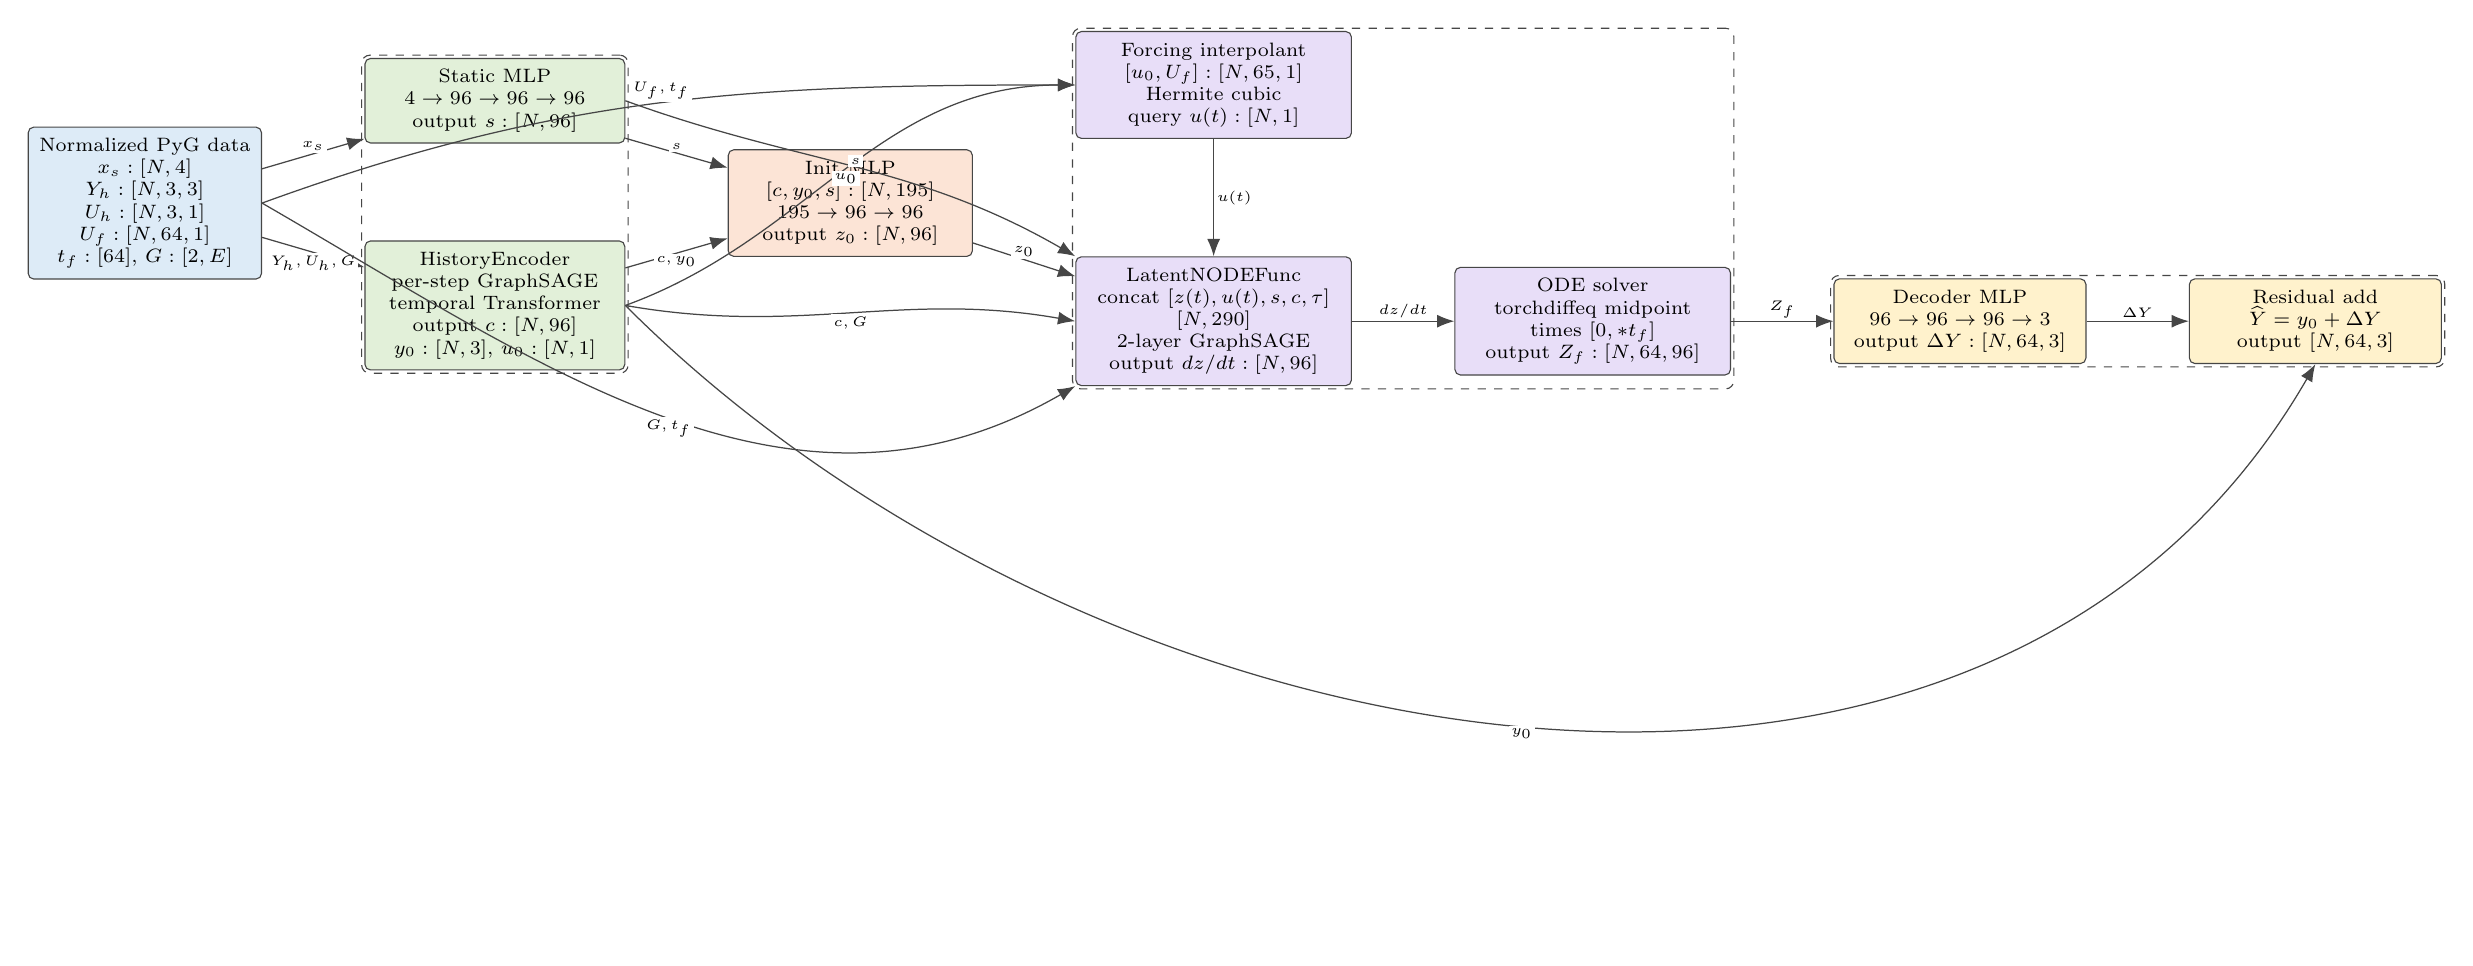
\begin{tikzpicture}[node distance=10mm and 13mm]
  \node[input] (data) {Normalized PyG data\\
    $x_s:[N,4]$\\
    $Y_h:[N,3,3]$\\
    $U_h:[N,3,1]$\\
    $U_f:[N,64,1]$\\
    $t_f:[64]$, $G:[2,E]$};

  \node[hist, right=of data, yshift=13mm] (static) {Static MLP\\
    $4 \rightarrow 96 \rightarrow 96 \rightarrow 96$\\
    output $s:[N,96]$};

  \node[hist, right=of data, yshift=-13mm] (history) {HistoryEncoder\\
    per-step GraphSAGE\\
    temporal Transformer\\
    output $c:[N,96]$\\
    $y_0:[N,3]$, $u_0:[N,1]$};

  \node[latent, right=of static, yshift=-13mm] (init) {Init MLP\\
    $[c,y_0,s]:[N,195]$\\
    $195 \rightarrow 96 \rightarrow 96$\\
    output $z_0:[N,96]$};

  \node[ode, right=of init, yshift=15mm] (control) {Forcing interpolant\\
    $[u_0,U_f]:[N,65,1]$\\
    Hermite cubic\\
    query $u(t):[N,1]$};

  \node[ode, right=of init, yshift=-15mm] (func) {LatentNODEFunc\\
    concat $[z(t),u(t),s,c,\tau]$\\
    $[N,290]$\\
    2-layer GraphSAGE\\
    output $dz/dt:[N,96]$};

  \node[ode, right=of func] (solver) {ODE solver\\
    torchdiffeq midpoint\\
    times $[0,*t_f]$\\
    output $Z_f:[N,64,96]$};

  \node[decode, right=of solver] (decoder) {Decoder MLP\\
    $96 \rightarrow 96 \rightarrow 96 \rightarrow 3$\\
    output $\Delta Y:[N,64,3]$};

  \node[decode, right=of decoder] (resid) {Residual add\\
    $\widehat{Y}=y_0+\Delta Y$\\
    output $[N,64,3]$};

  \draw[arrow] (data) -- node[label, above] {$x_s$} (static);
  \draw[arrow] (data) -- node[label, below] {$Y_h,U_h,G$} (history);
  \draw[arrow] (static) -- node[label, above] {$s$} (init);
  \draw[arrow] (history) -- node[label, below] {$c,y_0$} (init);
  \draw[arrow] (data.east) to[out=20,in=180] node[label, above] {$U_f,t_f$} (control.west);
  \draw[arrow] (history.east) to[out=20,in=180] node[label, below] {$u_0$} (control.west);
  \draw[arrow] (init) -- node[label, above] {$z_0$} (func);
  \draw[arrow] (control) -- node[label, right] {$u(t)$} (func);
  \draw[arrow] (static.east) to[out=-20,in=150] node[label, above] {$s$} (func.north west);
  \draw[arrow] (history.east) to[out=-10,in=170] node[label, below] {$c,G$} (func.west);
  \draw[arrow] (data.east) to[out=-30,in=210] node[label, below] {$G,t_f$} (func.south west);
  \draw[arrow] (func) -- node[label, above] {$dz/dt$} (solver);
  \draw[arrow] (solver) -- node[label, above] {$Z_f$} (decoder);
  \draw[arrow] (decoder) -- node[label, above] {$\Delta Y$} (resid);
  \draw[arrow] (history.east) to[out=-45,in=-120] node[label, below] {$y_0$} (resid.south);

  \begin{scope}[on background layer]
    \node[group, fit=(static)(history), label={[font=\scriptsize]above:HistoryEncoder}] {};
    \node[group, fit=(control)(func)(solver), label={[font=\scriptsize]above:Controlled latent ODE}] {};
    \node[group, fit=(decoder)(resid), label={[font=\scriptsize]above:Decoder}] {};
  \end{scope}
\end{tikzpicture}%
}
\caption*{Full NODE2 forward pass. All tensors are node-major. $G$ denotes edge\_index; $\tau=\mathrm{clamp}(t/t_f[-1],0,1)$.}
\end{figure}

\vspace{2mm}
\begin{figure}[h!]
\centering
\resizebox{0.95\textwidth}{!}{%
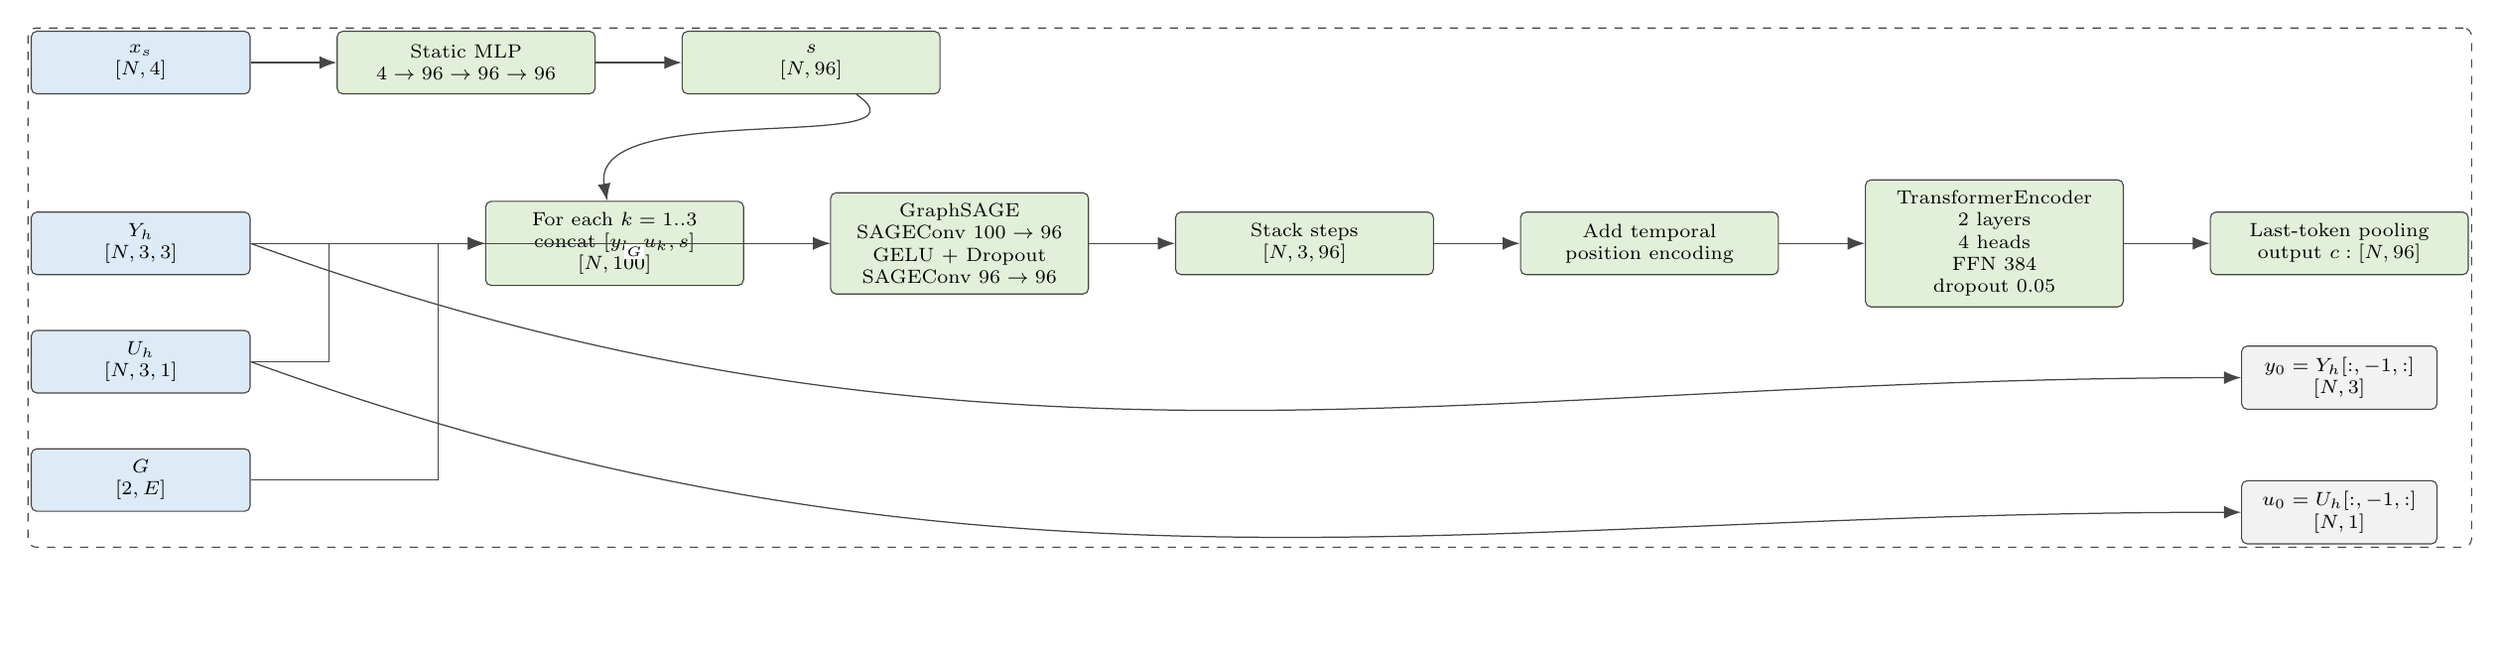
\begin{tikzpicture}[node distance=9mm and 11mm]
  \node[input] (xs) {$x_s$\\$[N,4]$};
  \node[hist, right=of xs] (smlp) {Static MLP\\$4\to96\to96\to96$};
  \node[hist, right=of smlp] (semb) {$s$\\$[N,96]$};

  \node[input, below=15mm of xs] (yh) {$Y_h$\\$[N,3,3]$};
  \node[input, below=7mm of yh] (uh) {$U_h$\\$[N,3,1]$};
  \node[input, below=7mm of uh] (g) {$G$\\$[2,E]$};

  \node[hist, right=30mm of yh] (concat) {For each $k=1..3$\\
    concat $[y_k,u_k,s]$\\
    $[N,100]$};
  \node[hist, right=of concat] (stepgnn) {GraphSAGE\\
    SAGEConv $100\to96$\\
    GELU + Dropout\\
    SAGEConv $96\to96$};
  \node[hist, right=of stepgnn] (stack) {Stack steps\\
    $[N,3,96]$};
  \node[hist, right=of stack] (pe) {Add temporal\\position encoding};
  \node[hist, right=of pe] (tr) {TransformerEncoder\\
    2 layers\\
    4 heads\\
    FFN 384\\
    dropout 0.05};
  \node[hist, right=of tr] (pool) {Last-token pooling\\
    output $c:[N,96]$};

  \node[small, below=9mm of pool] (lasts) {$y_0=Y_h[:,-1,:]$\\$[N,3]$};
  \node[small, below=9mm of lasts] (lastu) {$u_0=U_h[:,-1,:]$\\$[N,1]$};

  \draw[arrow] (xs) -- (smlp);
  \draw[arrow] (smlp) -- (semb);
  \draw[arrow] (yh) -- (concat);
  \draw[arrow] (uh.east) -- ++(10mm,0) |- (concat);
  \draw[arrow] (semb) to[out=-35,in=100] (concat);
  \draw[arrow] (g.east) -- ++(24mm,0) |- node[label, near end, below] {$G$} (stepgnn);
  \draw[arrow] (concat) -- (stepgnn);
  \draw[arrow] (stepgnn) -- (stack);
  \draw[arrow] (stack) -- (pe);
  \draw[arrow] (pe) -- (tr);
  \draw[arrow] (tr) -- (pool);
  \draw[arrow] (yh.east) to[out=-20,in=180] (lasts.west);
  \draw[arrow] (uh.east) to[out=-20,in=180] (lastu.west);

  \begin{scope}[on background layer]
    \node[group, fit=(xs)(smlp)(semb)(yh)(uh)(g)(concat)(stepgnn)(stack)(pe)(tr)(pool)(lasts)(lastu),
      label={[font=\scriptsize]above:HistoryEncoder detail}] {};
  \end{scope}
\end{tikzpicture}%
}
\caption*{HistoryEncoder detail. Spatial message passing is applied independently at each history step; temporal attention is per node over the $H=3$ tokens.}
\end{figure}

\newpage
\begin{center}
{\Large NODE2 Layer Table}
\end{center}

\renewcommand{\arraystretch}{1.2}
\begin{tabular}{p{0.18\textwidth} p{0.20\textwidth} p{0.41\textwidth} p{0.14\textwidth}}
\toprule
Module & Input & Layers & Output \\
\midrule
Static MLP & $[N,4]$ & Linear $4\to96$, GELU, Dropout 0.05; Linear $96\to96$, GELU, Dropout 0.05; Linear $96\to96$ & $[N,96]$ \\
History concat & $[N,3]$, $[N,1]$, $[N,96]$ & concat per history step & $[N,100]$ \\
History GraphSAGE & $[N,100]$, $G$ & SAGEConv $100\to96$, GELU, Dropout 0.05; SAGEConv $96\to96$ & $[N,96]$ \\
Temporal Transformer & $[N,3,96]$ & sinusoidal PE; 2 encoder layers; 4 heads; FFN 384; dropout 0.05 & $[N,3,96]$ \\
History pooling & $[N,3,96]$ & last token, identity projection & $c:[N,96]$ \\
Init MLP & $[c,y_0,s]=[N,195]$ & Linear $195\to96$, GELU; Linear $96\to96$ & $z_0:[N,96]$ \\
Forcing path & $[u_0,U_f]=[N,65,1]$, $t=[65]$ & Hermite cubic with backward differences & $u(t):[N,1]$ \\
Latent ODE func & $[z,u(t),s,c,\tau]=[N,290]$ & SAGEConv $290\to96$, Softplus; SAGEConv $96\to96$ & $dz/dt:[N,96]$ \\
ODE solver & $z_0:[N,96]$, $t=[65]$ & torchdiffeq midpoint, rtol $10^{-4}$, atol $10^{-5}$ & $Z_f:[N,64,96]$ \\
Decoder MLP & $[N,64,96]$ & Linear $96\to96$, GELU; Linear $96\to96$, GELU; Linear $96\to3$ & $\Delta Y:[N,64,3]$ \\
Residual output & $\Delta Y$, $y_0$ & $\widehat{Y}=y_0+\Delta Y$ & $[N,64,3]$ \\
\bottomrule
\end{tabular}

\end{document}
